\documentclass{article}
\usepackage{graphicx}
\usepackage{subcaption}
\graphicspath{ {figures/} }
\begin{document}

\section*{Abstract}
Transfer learning is a popular method for tackling machine learning problems with image classification, 
pre-trained models allows people to leverage it's generalization capabilities without needing large compute 
resources. In this project, we focused on models to classify images of mixed patterns of proteins,
taken with a microscope. To achieve this goal, we utilized transfer learning 
and demonstrated the hypothesis that earlier layers in a convolutional network captures simple features,
while later layers captures more complex features. Due to the differences between the training set
of the pre-trained model and our dataset, we show that earlier layers in a pre-trained convolutional network
gives better results in our classification task. Our best model realized a 94\% accuracy on 
the test dataset with limited computational sources, thus provided a feasible way for people with 
no powerful machines.
\section{Introduction}
There are now many neural network methods and architectures designed for 
image classification that perform exceptionally well. These models were trained
on millions of images, with powerful GPU acceleration. However in many cases where
an individual or group needs a model for an image classification task, these pre-trained
models do cannot be applied directly. In this case, the usual solution is to use transfer learning.
Using the pre-trained model as a feature extractor, we pass our task specific data into a 
pre-trained model and then train a linear classifier using the extracted features of our images.

These pre-trained models are usually trained on the ImageNet dataset\cite{imagenet_cvpr09}. This dataset is a large
collection of images of real world objects such as animals, like dogs and cats, and other objects like cars.
Thus we would expect these models to be good at extracting features from images that are similar to ImageNet,
aka real world, everyday objects. If we want to apply these models to images that are very different from 
the ImageNet dataset, such as the Human Protein dataset, we would expect the model to 
not be able to extract very good features.

\subsection{Human Protein Dataset}
\begin{figure}[h!]
    \centering
    \begin{subfigure}[b]{0.2\linewidth}
      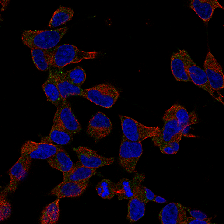
\includegraphics[width=\linewidth]{../../data/train/0a2abec8-bbb7-11e8-b2ba-ac1f6b6435d0.png}
    \end{subfigure}
    \begin{subfigure}[b]{0.2\linewidth}
      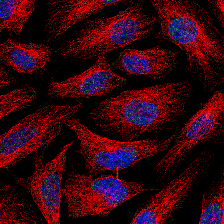
\includegraphics[width=\linewidth]{../../data/train/0a6068e8-bbb7-11e8-b2ba-ac1f6b6435d0.png}
    \end{subfigure}
    \begin{subfigure}[b]{0.2\linewidth}
        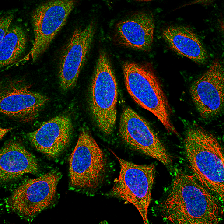
\includegraphics[width=\linewidth]{../../data/train/0a74debc-bbc2-11e8-b2bb-ac1f6b6435d0.png}
    \end{subfigure}
    \begin{subfigure}[b]{0.2\linewidth}
        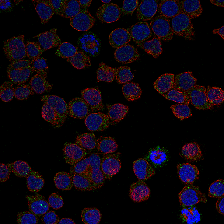
\includegraphics[width=\linewidth]{../../data/train/0bac19d6-bbc1-11e8-b2bb-ac1f6b6435d0.png}
    \end{subfigure}

    \begin{subfigure}[b]{0.2\linewidth}
        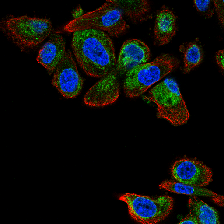
\includegraphics[width=\linewidth]{../../data/train/0ea71d6c-bbb1-11e8-b2ba-ac1f6b6435d0.png}
      \end{subfigure}
      \begin{subfigure}[b]{0.2\linewidth}
        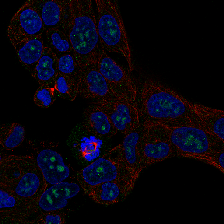
\includegraphics[width=\linewidth]{../../data/train/1a490006-bbaf-11e8-b2ba-ac1f6b6435d0.png}
      \end{subfigure}
      \begin{subfigure}[b]{0.2\linewidth}
          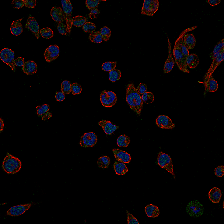
\includegraphics[width=\linewidth]{../../data/train/1e48964e-bbb4-11e8-b2ba-ac1f6b6435d0.png}
      \end{subfigure}
      \begin{subfigure}[b]{0.2\linewidth}
          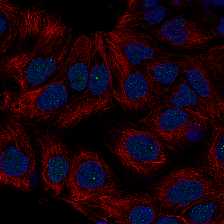
\includegraphics[width=\linewidth]{../../data/train/fcb70c22-bbc2-11e8-b2bc-ac1f6b6435d0.png}
      \end{subfigure}
    \caption{Example images from the Human Protein dataset}
  \end{figure}
  
Researches in the biology field have been made a lot easier by applying data analysis nowadays. Training machines for tedious work is saving experts a lot of time and also makes it possible to learn a mass of variations thoroughly. Specifically for protein study, an application is classifying well-known proteins, which is essential for learning a novel protein based on the group to which it is predicted to belong\cite{subcellular}. 

Historical efforts have been limited to single patterns in one or a few cell types, but in order to obtain a full understanding of the human cell, models are needed to classify mixed patterns across a range of different human cells. To address similar problems, people have tried adaptive k-NN classifiers\cite{knn}, support vector machines\cite{svm}, and decision trees\cite{dtree}. Though it was a breakthrough, the results they are getting is not so good compared to machine learning methods in recent years. A study conducted by the HPA Cell Atlas team\cite{nature}, with Devin Sullivan and Casper Winsnes as lead authors combined citizen science task and deep learning. The contribution of this study is huge. It not only achieved a good classification with the F1 score equal to 0.72 but also supplemented HPA Cell data with the result of gamers’ annotations. The data we are using is based on their supplements.

Though the HPA Cell Atlas team used the transfer-learning approach as well, their input involved the results of training 60,000 players and millions of images which is time-consuming and not applicable for small intuitions. So we proposed a project to classify proteins with pre-trained models.

  
\subsection{Transfer Learning}
\begin{figure}[h!]
  \centering
  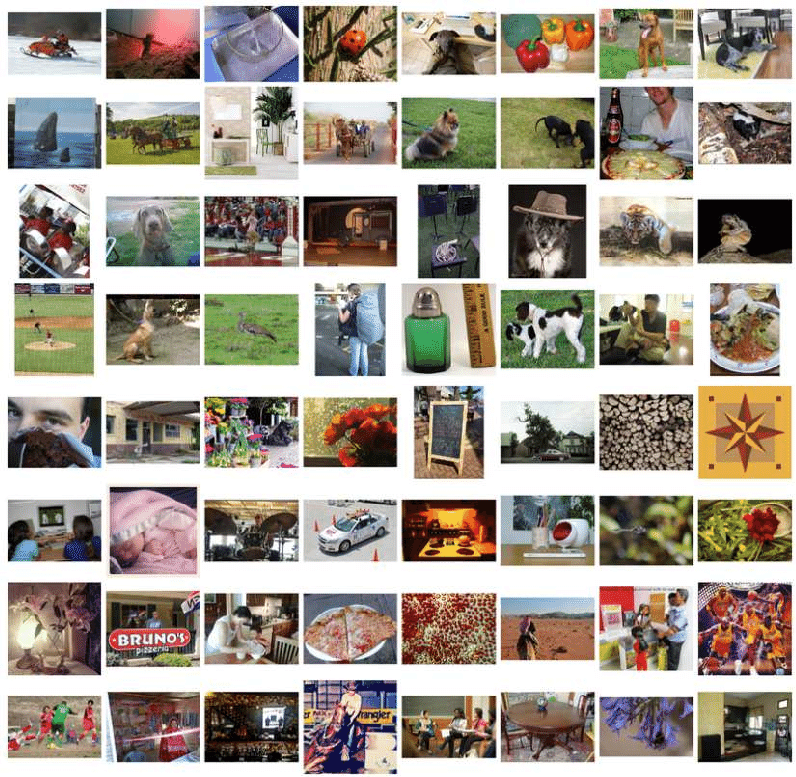
\includegraphics[scale=0.40]{Examples-in-the-ImageNet-dataset.png}
  \caption{Example images in the ImageNet dataset}
\end{figure}

It has been shown that in a deep convolutional neural network trained for image classification, the models
can be used on other image datasets to extract useful feature maps for machine learning purposes. The learned 
feature maps of the pre-trained network start very simple, looking for edges and corners, and become increasingly
complex as the layers get deeper.\cite{10.1007/978-3-319-10590-1_53} These learned feature maps are general enough to be applied to unseen data from 
from other image datasets\cite{NIPS2014_5347}.

The most common and powerful pre-trained models used for images are all trained on the ImageNet dataset\cite{imagenet_cvpr09}. This dataset
is an incredibly diverse set of images containing a thousand different classes of everyday objects. For most machine learning
applications relating to image processing, this dataset works very well as a base dataset for pre-trained networks as it can 
be interpreted as a superset of the images that an application would see in the real world. However, this is not true for all
applications, specifically those which deal with images that are very different from what we see in our everyday lives, for Example
images of microscopic objects.

The Human Protein Dataset is an example of such a dataset. They do not have much of the complex features that any real world image would have, and are mostly made up of 
lines, and circles and corners. Therefore we predict that early layers from a pre-trained model will
provide good features for classification for this dataset, while later layers will perform comparatively worse, 
due to the fact that the more complex patterns that the later layers are looking for do not exist in this 
dataset. 

In this paper we test this hypothesis by using a pre-trained model as a feature extractor, we choose multiple different
hidden layers from this model, and train a classifier on each different layer. We find that the best performing classifier
for the Human Protein dataset is the one with the earliest layer hidden layer as its feature extractor.
\section{Method}
We are seeking to test the feature extraction power of pre-trained networks on 
a dataset that is very different from the one which it is trained on. We take 
a pre-trained, state-of-the-art image classification model, ResNet50V2 \cite{DBLP:journals/corr/HeZR016}, and take
the feature maps of the model at different levels to use as the features for 
a linear classifier, which we train on our human protein data. We freeze the weights
of the pre-trained model and train only the added layers at the end.
\subsection{Data}
Our data consists of RGB images of human proteins, we process these into 3x224x224 sized
arrays as the input to our model. There are a total of 28 different possible classes,
and each image can belong to multiple classes. We process the labels to be "multi-hot":
a vector of length $n$ where $n$ is the number of classes, where it is a 1 at position $i$ if 
it belongs to the $i^{th}$ class and 0 otherwise.
\subsection{Model}

The input of our model consists of 224x224x3 sized arrays, they first go through a batch normalization layer\cite{ioffe2015batch}. This helps
us normalize the input to the pre-trained model on our specific dataset, allowing us 
to feed the raw data in without much preprocessing.

The ResNet50V2 model is conveniently structured as distinct residual blocks.
For our experiments we picked the outputs of 4 different residual blocks, evenly spaced between each other, in the model
as our final feature map. The output of the chosen hidden layers is a large amount of 
feature maps. Due to limitations of our compute resources, we chose not to directly flatten the feature maps and connect it to a dense prediction
layer due to the amount of feature maps ResNet50V2 outputs and thus the amount of parameters that would need. We chose to reduce the number of 
feature maps from the output by first passing it through a 1x1 convolution layer\cite{szegedy2014going} with 
Relu activation. This allows us to reduce the number of final feature maps in an efficient way, significantly reducing the number of parameters and training time. We then flatten the feature maps using global average pooling\cite{Lin2013NetworkIN}, and then connect to a 
fully connected dense layer for prediction. 

The dataset we are tackling is a multi label classification problem, therefore use sigmoid activation
in the prediction layer as each image can belong in multiple classes. We  use binary cross entropy as the loss function. 
\begin{equation}
    L(Y, \hat{Y}) = \sum_i^n y_i\log{(\hat{y}_i)}
\end{equation}
Where $Y$ is the "multi hot" representation of our label, $y_i$
is the value at each $i^{th}$ position in the label.  We assume that for every value in the output vector $\hat{y_i}$ is the probability
that an image is in class $i$, where each $\hat{y}_i$ is independent of other class probabilities because 
each $x$ can belong to multiple classes at the same time. 

\subsection{Training}
To train the each model we used the ADAM optimization algorithm\cite{kingma2014adam} with mini-batches of size 32.
The parameters we used for ADAM were: $\eta = 10^{-3}$, $\beta_1 = 0.9$, $beta_2=0.999$, these
are the default values in Keras' implementation of ADAM.
We were able to run 10 epochs of training on each model given our computing resources. 
\section{Results}
Comparing the results of the models, we found the pre-trained model with the earliest hidden layer performed the best, with the accuracy rate on the test dataset equal to 0.946. This is consistent with our guess as the earlier layer focuses on the basic features of images, such as lines and shapes. Since the images of protein are composed of similar shapes and simple colors, the earlier layer could capture the variance better. 

\begin{table}[h!]
\centering

\begin{tabular}{|c|c|c|c|c|}
    \hline\\
     Model1 & Model2&Model3&Model4 \\
     \hline\\
     Error&0.229&0.565&0.314&0.236\\
     \hline\\
     Accuracy&0.946&0.932&0.927&0.936\\
      \hline
     F1 Score&0.321&0.169&0.312&0.267\\
     \hline
\end{tabular}

{\raggedright Table 1: Results of models on test set. Above is the result of models, where Model1 represents the pre-trained model with the earliest layer, Model2 with the second earliest layer and so on. \par}

\label{table:1}
\end{table}

What is more, we predict the classes based on the threshold that the probabilities of chosen classes have to be larger than twice the probabilities of unchosen classes and calculated the F1 score on the test data. The data is very unbalanced, with the largest class counting for 42\% of the training data and getting an F1 score of 0.680 on the test data. So we choose the weighted F1 score and that of the best model is 0.32. We noticed that judging on F1 score, our model performance is not good compared to that of the HPA Cell Atlas team's study. It is possibly caused by the unbalance in data and the limited number of trained epochs.

Considering we are able to finish training this model on 26455 images in 4 hours, this result is pretty applicable in practice.

\newpage
\bibliography{paper}
\bibliographystyle{ieeetr}
\end{document}



